\documentclass[dvisvgm]{beamer}
\usepackage{tikz}
\usepackage{animate}
\usetikzlibrary{animations}
\begin{document}
% 制作animate,需要满足以下条件:
% 1.使用beamer类的documentclass,并且携带dvisvgm参数
% 2.使用animations库
% 3.使用texlive编译命令: latexmk -pdflatex -dvi <tex_file>
% 4.dvi文件转化为svg命令: dvisvgm <dvi_file>
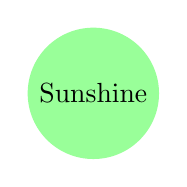
\begin{tikzpicture}
    % fill opacity/rotate代表该动画变化的属性
    % 0s/2s/4s代表不同时间点属性状态,为关键帧
    % base代表在动画激活时间外的属性值,默认为node属性值,提供该选项后覆盖node属性值. 可使用方案列表:
    %   1)base - 动画激活时间之外的属性值
    %   2)forever - 保持动画最后的属性值
    %   3)freeze - 类似于forever
    \path node[fill=green!40,circle] at (0,0) :fill opacity={0s="1",2s="0",4s="1",repeats=2} :rotate={0s="0",2s="180",4s="360",repeats} {Sunshine};
\end{tikzpicture}\\\vspace{1cm}


\begin{tikzpicture}
    % begin on=click代表由点击动作开始动画. 可选方案列表:
    %   1)begin - 从绝对0s相对向前(<-)偏移指定秒开始计时, 绝对时间为0-begin
    %   2)end - 相对于begin时间的偏移时间结束, 绝对时间为end-begin
    %   3)begin on - 动作触发动画开始, 每一次动作都会让动画重新开始. 动作列表如下:
    %     [1]click - 鼠标的点击和释放操作
    %     [2]mouse down - 鼠标的点击操作
    %     [3]mouse up - 鼠标的释放操作
    %     [4]mouse over - 鼠标放置在node上
    %     [5]mouse move - 鼠标放置在node上, 并且移动
    %     [6]mouse out - 鼠标从node上, 移动到node范围外
    %     [7]begin - 跟随当前node的其他动作激活而激活(需等待其他动作结束), 配合of next指定其他动作的名称
    %     [8]begin - 跟随当前node的其他动作结束而结束, 配合of next指定其他动作的名称
    %   4)repeats - 动画重复指定次数. 值列表如下:
    %     [1]没有指定值 - 默认重复无限次数
    %     [2]指定具体值 - 重复指定次数
    %     [3]accumulating - 在动画结束后, 不复位进行动画,使动画效果叠加
    %   5)restart - bool类型(true/false), 动画是否能够重启
    \path node[draw,line width=2pt,fill=green] at (0,0) :rotate={1s="0",5s="90",forever,begin on={begin,end,of next=X}} :draw={1s="blue",5s="purple",begin on={click},name=X} {Click me!};
\end{tikzpicture}\\\vspace{1cm}
    

\begin{tikzpicture}
    \path node[fill=green] at (0,0) :fill={0s="red",2s="blue",forever,begin on=click} {Click me!};
\end{tikzpicture}
\end{document}
